\documentclass[11pt,a4paper]{article}
\usepackage[utf8]{inputenc}
\usepackage{amsmath,amssymb}
\usepackage{geometry}
\geometry{left=25mm,right=20mm,top=25mm,bottom=25mm}
\usepackage{enumitem}
\usepackage{multicol}
\usepackage{tikz,pgfplots}
\pgfplotsset{compat=1.18}
\usepackage{fancyhdr}
\usepackage[hidelinks]{hyperref}
\setlength{\parindent}{0pt}
\setlength{\parskip}{6pt}
\newcommand{\jawab}{\par\medskip\textbf{Penyelesaian.}\par}
\newcommand{\R}{\mathbb{R}}
\newcommand{\catatan}[1]{\par\smallskip\textbf{Catatan.} #1\par}

\begin{document}

\section*{Latihan 2.4}
\begin{enumerate}
    \item[5.] Dapatkan rumus untuk $f^{-1}$ dan sebutkan domainnya.
\begin{enumerate}
    \item $f(x)=x^4+2$, $x\geq 0$.
    \item $f(x)=-\sqrt{2-7x}$.
    \item $f(x)=\sqrt{x+6}$.
    \item $f(x)=-\sqrt{3-2x}$.
\end{enumerate}
\jawab
Domain $f^{-1}$ adalah range $f$. Untuk mencari invers, tuliskan $y=f(x)$,
selesaikan untuk $x$, lalu tukar nama variabel $x$ dan $y$.
\begin{enumerate}
    \item Dari $y=x^4+2$ dengan $x\geq 0$, diperoleh
    \[
        x=\sqrt[4]{y-2}.
    \]
    Karena $x^4\geq 0$, range $f$ adalah $[2,\infty)$. Jadi,
    \[
        \boxed{f^{-1}(x)=\sqrt[4]{x-2},\qquad D_{f^{-1}}=[2,\infty).}
    \]

    \item Syarat akar memberikan $2-7x\geq 0$, yaitu $x\leq 2/7$.
    Karena $y=-\sqrt{2-7x}\leq 0$, range $f$ adalah $(-\infty,0]$.
    Selanjutnya,
    \[
        y^2=2-7x\quad\Longrightarrow\quad x=\frac{2-y^2}{7}.
    \]
    Dengan demikian,
    \[
        \boxed{f^{-1}(x)=\frac{2-x^2}{7},\qquad D_{f^{-1}}=(-\infty,0].}
    \]

    \item Domain $f$ adalah $[-6,\infty)$ dan range-nya $[0,\infty)$.
    Dari $y=\sqrt{x+6}$ diperoleh $y^2=x+6$, sehingga
    \[
        \boxed{f^{-1}(x)=x^2-6,\qquad D_{f^{-1}}=[0,\infty).}
    \]

    \item Domain $f$ adalah $(-\infty,3/2]$ dan range-nya $(-\infty,0]$.
    Dari $y=-\sqrt{3-2x}$ diperoleh $y^2=3-2x$, sehingga
    \[
        \boxed{f^{-1}(x)=\frac{3-x^2}{2},\qquad D_{f^{-1}}=(-\infty,0].}
    \]
\end{enumerate}
\item[9.] Diberikan fungsi $f(x)=a+\sqrt{x-b}$ dan $g(x)=(x-a)^2+b$ untuk sebarang
bilangan real $a$ dan $b$.
\begin{enumerate}
    \item Dapatkan domain dan range dari $f(x)$.
    \item Dapatkan domain $g(x)$ agar fungsi $f(x)$ dan $g(x)$ saling invers.
    Jelaskan jawaban Anda!
    \item Sketsa kurva $f(x)$ dan $f^{-1}(x)$ dalam satu bidang koordinat.
\end{enumerate}

\jawab
\begin{enumerate}
    \item Syarat $x-b\geq 0$ memberikan $x\geq b$. Karena
    $\sqrt{x-b}\geq 0$, nilai $f(x)$ memenuhi $f(x)\geq a$, dan setiap nilai
    $y\geq a$ dapat dicapai. Jadi,
    \[
        \boxed{D_f=[b,\infty),\qquad R_f=[a,\infty).}
    \]

    \item Domain $g$ harus sama dengan range $f$, yaitu
    \[
        \boxed{D_g=[a,\infty).}
    \]
    Untuk $x\geq b$,
    \[
        g(f(x))=\bigl(a+\sqrt{x-b}-a\bigr)^2+b=x.
    \]
    Untuk $x\geq a$,
    \[
        f(g(x))=a+\sqrt{(x-a)^2}=a+|x-a|=x.
    \]
    Pembatasan $x\geq a$ diperlukan karena untuk $x<a$ ekspresi terakhir
    menjadi $2a-x$, bukan $x$. Maka
    \[
        \boxed{f^{-1}(x)=(x-a)^2+b,\qquad x\geq a.}
    \]

    \item Grafik $f$ dimulai dari $(b,a)$, naik, dan cekung ke bawah.
    Grafik invers dimulai dari $(a,b)$ dan merupakan bagian kanan parabola
    $y=(x-a)^2+b$. Kedua grafik saling mencerminkan terhadap garis $y=x$.
    Untuk sebarang $a,b$, titik-titik pada kedua grafik dapat digambar dengan
    parameter $t\geq 0$:
    \[
        \begin{array}{c|c}
            \text{Grafik }f & \text{Grafik }f^{-1}\\ \hline
            (b+t^2,\ a+t) & (a+t,\ b+t^2)
        \end{array}
    \]
    Sebagai ilustrasi, berikut sketsa untuk $a=1$ dan $b=-1$.
    Nilai parameter lain mengubah letak kedua titik awal sesuai rumus di atas.
    \begin{center}
    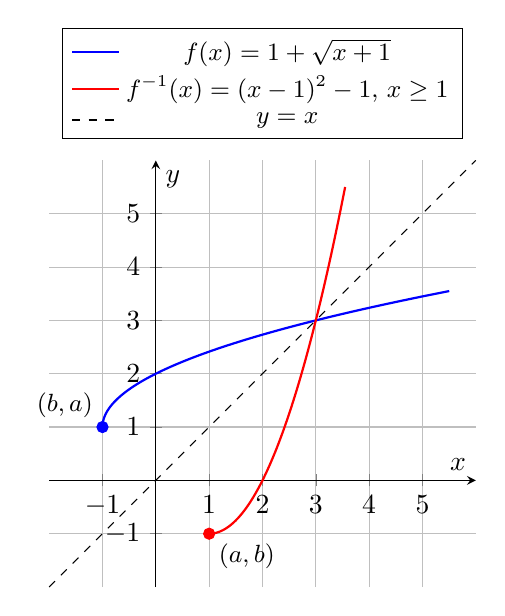
\begin{tikzpicture}
        \begin{axis}[
            width=10cm,height=7cm,axis equal image,clip=false,
            axis lines=middle,xmin=-2,xmax=6,ymin=-2,ymax=6,
            xlabel={$x$},ylabel={$y$},grid=both,
            xtick={-1,0,1,2,3,4,5},ytick={-1,0,1,2,3,4,5},
            legend style={at={(0.5,1.05)},anchor=south,font=\small}
        ]
            \addplot[blue,thick,domain=0:2.55,samples=100]
                ({-1+x^2},{1+x});
            \addlegendentry{$f(x)=1+\sqrt{x+1}$}
            \addplot[red,thick,domain=0:2.55,samples=100]
                ({1+x},{-1+x^2});
            \addlegendentry{$f^{-1}(x)=(x-1)^2-1$, $x\geq 1$}
            \addplot[black,dashed,domain=-2:6] {x};
            \addlegendentry{$y=x$}
            \addplot[only marks,mark=*,blue] coordinates {(-1,1)};
            \addplot[only marks,mark=*,red] coordinates {(1,-1)};
            \node[above left,font=\small] at (axis cs:-1,1) {$(b,a)$};
            \node[below right,font=\small] at (axis cs:1,-1) {$(a,b)$};
        \end{axis}
    \end{tikzpicture}
    \end{center}
\end{enumerate}

\item[15.] Diketahui $f(t)=3t^2-5t+6$. Jika $f^{-1}(t_0)=1$, maka $f(t_0)=\ldots$
\begin{multicols}{5}
    \begin{enumerate}[label=(\Alph*)]
    \item -4
    \item -1
    \item 14
    \item 34
    \item 74
\end{enumerate}
\end{multicols}

\jawab
Dari sifat invers, $f^{-1}(t_0)=1$ berarti $t_0=f(1)$. Jadi,
\[
    t_0=3(1)^2-5(1)+6=4.
\]
Maka
\[
    f(t_0)=f(4)=3(4)^2-5(4)+6=48-20+6=\boxed{34}.
\]
Jawaban: \textbf{(D)}.\\
\catatan{Fungsi kuadrat ini tidak mempunyai invers sebagai fungsi jika
domainnya seluruh $\R$. Notasi $f^{-1}$ dalam soal mengandaikan pembatasan
domain yang membuat $f$ satu-satu dan memuat $t=1$, misalnya
$[5/6,\infty)$. Dengan asumsi tersebut, perhitungan di atas sah.}
\item[18.] 
Diberikan $f(x)=-\sqrt{4-7x}$. Dapatkan rumus untuk $f^{-1}$ dan sebutkan
domainnya.
\begin{enumerate}[label=(\Alph*)]
    \item $f^{-1}(x)=\dfrac{1}{7}(4-x^2)$, $x\leq 0$.
    \item $f^{-1}(x)=\dfrac{1}{7}(4+x^2)$, $x\leq 0$.
    \item $f^{-1}(x)=-\dfrac{1}{7}(4-x^2)$, $x\leq 0$.
    \item $f^{-1}(x)=-\dfrac{1}{7}(x^2-4)$, $x\leq 0$.
    \item $f^{-1}(x)=\dfrac{1}{7}(x^2+4)$, $x\leq 0$.
\end{enumerate}

\jawab
Domain $f$ diperoleh dari $4-7x\geq 0$, yaitu $(-\infty,4/7]$.
Range $f$ adalah $(-\infty,0]$. Dengan $y=-\sqrt{4-7x}$, diperoleh
\[
    y^2=4-7x\quad\Longrightarrow\quad x=\frac{4-y^2}{7}.
\]
Jadi,
\[
    \boxed{f^{-1}(x)=\frac{4-x^2}{7},\qquad D_{f^{-1}}=(-\infty,0].}
\]
\catatan{Pilihan \textbf{(A)} dan \textbf{(D)} sama-sama benar karena
$-\frac{1}{7}(x^2-4)=\frac{1}{7}(4-x^2)$. Dengan pilihan yang tercetak,
soal tidak memiliki satu jawaban pilihan ganda yang unik.}
\end{enumerate}

\section*{Latihan 3.1}
\begin{enumerate}

% Sumber: WhatsApp Image 2026-10-05 at 19.21.27 (2).jpeg
\item[6.] Grafik fungsi $f$ digambarkan berikut ini, dapatkan:
\begin{multicols}{2}
    \noindent
    \begin{center}
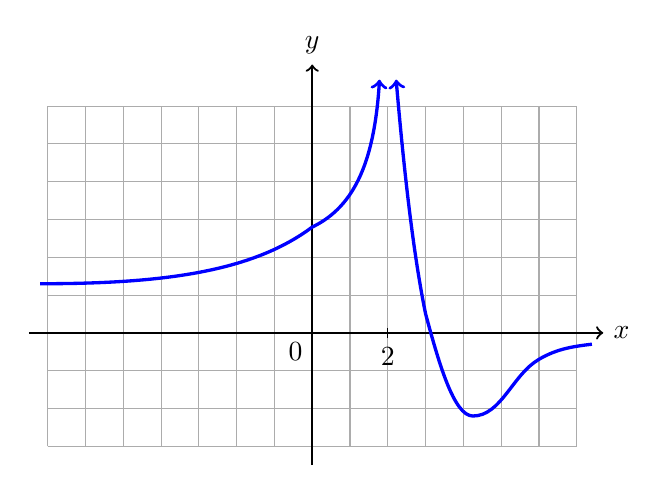
\begin{tikzpicture}[x=0.48cm,y=0.48cm]
    % Sketsa ulang grafik sumber; satu kotak menyatakan satu satuan.
    \draw[step=1,gray!65,thin] (-7,-3) grid (7,6);
    \draw[->,thick] (-7.5,0)--(7.7,0) node[right] {$x$};
    \draw[->,thick] (0,-3.5)--(0,7.1) node[above] {$y$};
    \node[below left] at (0,0) {$0$};
    \draw (2,0.13)--(2,-0.13) node[below] {$2$};
    \draw[very thick,blue,->]
        (-7.2,1.3) .. controls (-4,1.3) and (-1.6,1.6) .. (0,2.8)
        .. controls (1.15,3.35) and (1.65,4.6) .. (1.78,6.7);
    \draw[very thick,blue,<-]
        (2.22,6.7) .. controls (2.4,4.6) and (2.65,2.2) .. (3,0.5)
        .. controls (3.35,-0.8) and (3.75,-2.2) .. (4.25,-2.2)
        .. controls (5,-2.2) and (5.3,-1.1) .. (6,-0.7)
        .. controls (6.5,-0.4) and (7,-0.35) .. (7.4,-0.3);
\end{tikzpicture}
\end{center}
    \begin{enumerate}
    \item $\displaystyle\lim_{x\to 2^-}f(x)$.
    \item $\displaystyle\lim_{x\to 2^+}f(x)$.
    \item $\displaystyle\lim_{x\to 2}f(x)$.
    \item $f(2)$.
\end{enumerate}
\end{multicols}

\jawab
Saat $x$ mendekati $2$ dari kiri maupun kanan, grafik naik tanpa batas.
Garis $x=2$ merupakan asimtot tegak, dan tidak ada titik grafik yang
menyatakan nilai fungsi pada $x=2$.
\begin{enumerate}
    \item $\displaystyle\boxed{\lim_{x\to 2^-}f(x)=+\infty}$.
    \item $\displaystyle\boxed{\lim_{x\to 2^+}f(x)=+\infty}$.
    \item Karena kedua limit satu sisi menuju $+\infty$,
    $\displaystyle\boxed{\lim_{x\to 2}f(x)=+\infty}$.
    Ini menyatakan limit tak hingga; limit sebagai bilangan real hingga
    tidak ada.
    \item $\boxed{f(2)\text{ tidak terdefinisi}}$ berdasarkan grafik.
\end{enumerate}

\item[8.] Buatlah sketsa grafik yang mungkin untuk fungsi $f$ dengan syarat-syarat
berikut (banyak penyelesaian yang mungkin):
\begin{enumerate}
    \item Domain $f$ adalah $[-1,1]$.
    \item $f(-1)=f(0)=f(1)=0$.
    \item $\displaystyle
        \lim_{x\to -1^-}f(x)=\lim_{x\to 1^+}f(x)=\lim_{x\to 0}f(x)=1$.
\end{enumerate}

\jawab
\textbf{Untuk teks yang tercetak, tidak ada fungsi yang memenuhi semua
syarat.} Domain $[-1,1]$ tidak memuat titik di sebelah kiri $-1$ maupun
di sebelah kanan $1$. Karena itu, limit $x\to -1^-$ dan $x\to 1^+$
tidak dapat didefinisikan sebagai limit satu sisi pada domain tersebut.

\catatan{Kemungkinan arah limit pada kedua ujung interval tertukar.
Jika yang dimaksud adalah $x\to -1^+$ dan $x\to 1^-$, salah satu
penyelesaiannya adalah fungsi berikut. Koreksi ini merupakan interpretasi,
bukan perubahan pada transkripsi soal.}
\[
    f(x)=
    \begin{cases}
        1, & x\in(-1,0)\cup(0,1),\\
        0, & x\in\{-1,0,1\}.
    \end{cases}
\]
Domain fungsi tersebut tepat $[-1,1]$, dengan
\[
    f(-1)=f(0)=f(1)=0,\qquad
    \lim_{x\to -1^+}f(x)=\lim_{x\to 1^-}f(x)=\lim_{x\to 0}f(x)=1.
\]
Sketsa untuk \textbf{interpretasi arah limit yang dikoreksi}:
\begin{center}
\begin{tikzpicture}[x=3cm,y=2cm]
    \draw[->] (-1.35,0)--(1.4,0) node[right] {$x$};
    \draw[->] (0,-0.2)--(0,1.4) node[above] {$y$};
    \draw[blue,very thick] (-1,1)--(0,1)--(1,1);
    \foreach \x in {-1,0,1}{
        \draw[blue,thick,fill=white] (\x,1) circle[radius=2.4pt];
        \fill (\x,0) circle[radius=2.4pt];
    }
    \node[below] at (-1,0) {$-1$};
    \node[below left] at (0,0) {$0$};
    \node[below] at (1,0) {$1$};
    \node[above left] at (0,1) {$1$};
\end{tikzpicture}
\end{center}
Lingkaran kosong menunjukkan titik yang tidak termasuk grafik, sedangkan
titik penuh menunjukkan nilai fungsi.

% : WhatsApp Image 2026-10-05 at 19.21.28 (1).jpeg
\newpage
\item[15.] Diketahui fungsi $f$ dengan $f(-3)=f(2)=2$,
$\displaystyle\lim_{x\to 1}f(x)=f(0)=1$, dan
$\displaystyle\lim_{x\to 0^-}f(x)=\lim_{x\to 0^+}f(x)=-1$.
Sketsa grafik berikut ini yang merupakan grafik $y=f(x)$ adalah:

\catatan{Gambar sumber hanya memuat pernyataan soal; pilihan-pilihan
grafiknya tidak terlihat. Karena itu, huruf pilihan jawaban tidak dapat
ditentukan. Berikut satu contoh grafik yang memenuhi seluruh syarat.}

\jawab
Grafik yang benar harus memiliki titik penuh di $(-3,2)$, $(2,2)$, dan
$(0,1)$. Kedua cabang di sekitar $x=0$ harus mendekati $(0,-1)$, yang
ditandai dengan lingkaran kosong. Di sekitar $x=1$, grafik harus mendekati
ketinggian $1$ dari kedua sisi.

Salah satu fungsi yang memenuhi semua syarat adalah
\[
    f(x)=
    \begin{cases}
        -x-1, & x<0,\\
        1, & x=0,\\
        2x-1, & 0<x\leq 1,\\
        x, & x>1.
    \end{cases}
\]
Pemeriksaannya:
\[
    f(-3)=2,\qquad f(2)=2,\qquad f(0)=1,
\]
\[
    \lim_{x\to 0^-}f(x)=-1=\lim_{x\to 0^+}f(x),\qquad
    \lim_{x\to 1^-}f(x)=1=\lim_{x\to 1^+}f(x).
\]
\begin{center}
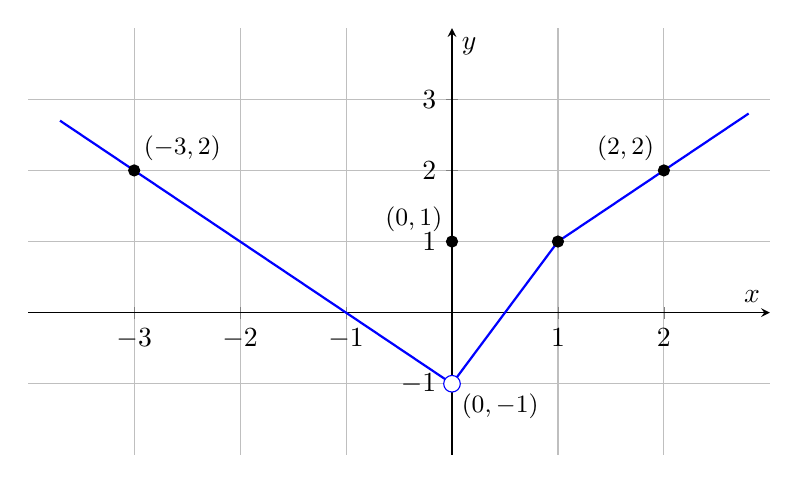
\begin{tikzpicture}
    \begin{axis}[
        width=11cm,height=7cm,axis lines=middle,
        xmin=-4,xmax=3,ymin=-2,ymax=4,
        xlabel={$x$},ylabel={$y$},grid=major,
        xtick={-3,-2,-1,0,1,2},ytick={-1,0,1,2,3}
    ]
        \addplot[blue,thick,domain=-3.7:0] {-x-1};
        \addplot[blue,thick,domain=0:1] {2*x-1};
        \addplot[blue,thick,domain=1:2.8] {x};
        \addplot[only marks,mark=*,black]
            coordinates {(-3,2) (2,2) (0,1) (1,1)};
        \addplot[only marks,mark=*,mark options={fill=white,draw=blue},
            mark size=3pt] coordinates {(0,-1)};
        \node[above right,font=\small] at (axis cs:-3,2) {$(-3,2)$};
        \node[above left,font=\small] at (axis cs:2,2) {$(2,2)$};
        \node[above left,font=\small] at (axis cs:0,1) {$(0,1)$};
        \node[below right,font=\small] at (axis cs:0,-1) {$(0,-1)$};
    \end{axis}
\end{tikzpicture}
\end{center}
Pada contoh ini dipilih $f(1)=1$, meskipun soal hanya mensyaratkan
$\lim_{x\to 1}f(x)=1$ dan tidak menetapkan nilai $f(1)$.
\end{enumerate}

\newpage
\section*{Latihan 3.2}
\begin{enumerate}

% Sumber: WhatsApp Image 2026-10-05 at 19.21.28 (2).jpeg
\item[4.] Dapatkan limit pada masing-masing soal berikut.
\begin{enumerate}
    \item[(b)] $\displaystyle\lim_{t\to -1}\frac{t^2+6t+5}{t^2-3t-4}$.
    \item[(d)] $\displaystyle\lim_{x\to 4^-}\frac{4-x}{2-\sqrt{x}}$.
    \item[(f)] $\displaystyle\lim_{y\to 1}y(y-1)(y+1)$.
    \item[(h)]$\displaystyle\lim_{x\to 0}\frac{12-3x^3+4x^7}{3x-24}$.
\end{enumerate}

\jawab
\begin{enumerate}
    \item[(b)] Faktorkan pembilang dan penyebut. Untuk $t\neq -1$ di sekitar
    $-1$,
    \[
        \frac{t^2+6t+5}{t^2-3t-4}
        =\frac{(t+1)(t+5)}{(t+1)(t-4)}=\frac{t+5}{t-4}.
    \]
    Maka
    \[
        \lim_{t\to -1}\frac{t^2+6t+5}{t^2-3t-4}
        =\frac{-1+5}{-1-4}=\boxed{-\frac45}.
    \]

    \item[(d)] Gunakan $4-x=(2-\sqrt{x})(2+\sqrt{x})$. Untuk $x\neq4$,
    \[
        \frac{4-x}{2-\sqrt{x}}=2+\sqrt{x}.
    \]
    Jadi,
    \[
        \lim_{x\to4^-}\frac{4-x}{2-\sqrt{x}}
        =2+\sqrt4=\boxed4.
    \]

    \item[(f)] Dengan kekontinuan polinomial,
    \[
        \lim_{y\to1}y(y-1)(y+1)=1(1-1)(1+1)=\boxed0.
    \]

    \item[(h)] Penyebut tidak nol pada $x=0$, sehingga
    \[
        \lim_{x\to0}\frac{12-3x^3+4x^7}{3x-24}
        =\frac{12}{-24}=\boxed{-\frac12}.
    \]
\end{enumerate}

\item[7.] Diberikan
\[
    f(x)=
    \begin{cases}
        \dfrac{x^3-8}{x-2}, & x\neq2,\\[6pt]
        k, & x=2.
    \end{cases}
\]
Tentukan nilai $k$ sehingga $\displaystyle\lim_{x\to2}f(x)=f(2)$ dan
kemudian nyatakan $f$ sebagai polinomial.

\jawab
Untuk $x\neq2$, faktorisasi selisih kubus memberikan
\[
    f(x)=\frac{(x-2)(x^2+2x+4)}{x-2}=x^2+2x+4.
\]
Dengan demikian,
\[
    \lim_{x\to2}f(x)=2^2+2(2)+4=12.
\]
Agar limit sama dengan $f(2)=k$, harus dipilih $\boxed{k=12}$.
Karena polinomial $x^2+2x+4$ juga bernilai $12$ pada $x=2$, diperoleh
\[
    \boxed{f(x)=x^2+2x+4\quad\text{untuk semua }x\in\R.}
\]

% Sumber: WhatsApp Image 2026-10-05 at 19.21.29 (1).jpeg, bagian atas
\item[10.] Diberikan $f(x)=\dfrac{x^3-1}{x-1}$.
\begin{enumerate}
    \item Dapatkan $\displaystyle\lim_{x\to1}f(x)$.
    \item Buatlah sketsa grafik $y=f(x)$.
\end{enumerate}

\jawab
\begin{enumerate}
    \item Untuk $x\neq1$,
    \[
        f(x)=\frac{(x-1)(x^2+x+1)}{x-1}=x^2+x+1.
    \]
    Karena itu,
    \[
        \boxed{\lim_{x\to1}f(x)=1^2+1+1=3.}
    \]

    \item Grafiknya adalah parabola
    \[
        y=x^2+x+1=\left(x+\frac12\right)^2+\frac34,
        \qquad x\neq1.
    \]
    Parabola membuka ke atas, berpuncak di $(-1/2,3/4)$, memotong
    sumbu $y$ di $(0,1)$, dan tidak memotong sumbu $x$. Titik $(1,3)$
    berupa lingkaran kosong karena fungsi asal tidak terdefinisi pada
    $x=1$. Domainnya $\R\setminus\{1\}$.
    \begin{center}
    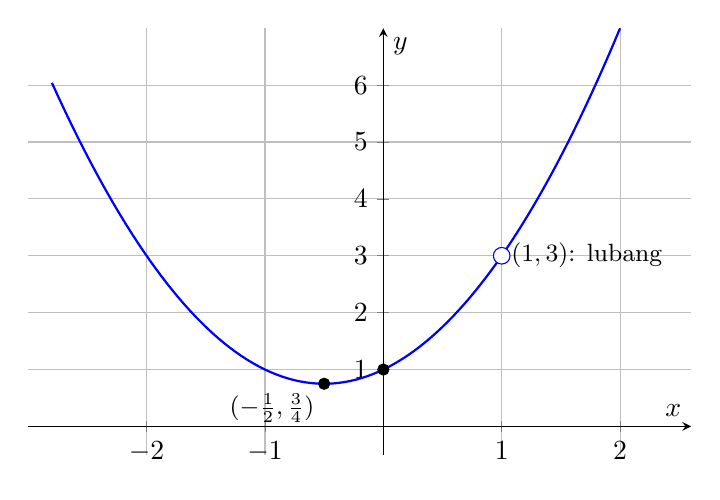
\begin{tikzpicture}
        \begin{axis}[
            width=10cm,height=7cm,axis lines=middle,
            xmin=-3,xmax=2.6,ymin=-0.5,ymax=7,
            xlabel={$x$},ylabel={$y$},grid=major,
            xtick={-2,-1,0,1,2},ytick={1,2,3,4,5,6}
        ]
            \addplot[blue,thick,domain=-2.8:2,samples=100] {x^2+x+1};
            \addplot[only marks,mark=*,mark options={fill=white,draw=blue},
                mark size=3pt] coordinates {(1,3)};
            \addplot[only marks,mark=*,black] coordinates {(-0.5,0.75) (0,1)};
            \node[right,font=\small] at (axis cs:1,3) {$(1,3)$: lubang};
            \node[below left,font=\small] at (axis cs:-0.5,0.75)
                {$(-\frac12,\frac34)$};
        \end{axis}
    \end{tikzpicture}
    \end{center}
\end{enumerate}

% Sumber: WhatsApp Image 2026-10-05 at 19.21.29 (1).jpeg, bagian bawah
\item[11.] Misalkan
\[
    f(x)=
    \begin{cases}
        \dfrac{x^2-9}{x+3}, & x>-3,\\[6pt]
        x-9, & x\leq-3.
    \end{cases}
\]
\begin{enumerate}
    \item Dapatkan $\displaystyle\lim_{x\to-3^+}f(x)$.
    \item Dapatkan $\displaystyle\lim_{x\to-3^-}f(x)$.
    \item Dapatkan $\displaystyle\lim_{x\to-3}f(x)$.
\end{enumerate}

\jawab
\begin{enumerate}
    \item Untuk $x>-3$, gunakan cabang pertama:
    \[
        f(x)=\frac{(x-3)(x+3)}{x+3}=x-3.
    \]
    Jadi,
    \[
        \boxed{\lim_{x\to-3^+}f(x)=-3-3=-6.}
    \]

    \item Untuk $x<-3$, gunakan cabang kedua:
    \[
        \boxed{\lim_{x\to-3^-}f(x)=\lim_{x\to-3^-}(x-9)=-12.}
    \]

    \item Kedua limit satu sisi berbeda, yaitu $-6\neq-12$. Maka
    \[
        \boxed{\lim_{x\to-3}f(x)\text{ tidak ada}.}
    \]
    Nilai fungsi pada titik tersebut adalah $f(-3)=-12$, tetapi nilai ini
    tidak membuat kedua limit satu sisi sama.
\end{enumerate}

% Sumber: WhatsApp Image 2026-10-05 at 19.21.29 (2).jpeg
\item[13.] Diberikan fungsi
\[
    f(x)=
    \begin{cases}
        \dfrac{\sqrt{x+9}-3}{x}, & x\neq0,\\[6pt]
        \dfrac13 k=\dfrac15, & x=0.
    \end{cases}
\]
Dapatkan nilai $k$ sehingga $\displaystyle\lim_{x\to0}f(x)=f(0)$.

\jawab
\begin{align*}
    \frac{\sqrt{x+9}-3}{x}
    &=\frac{(\sqrt{x+9}-3)(\sqrt{x+9}+3)}{x(\sqrt{x+9}+3)}\\
    &=\frac{x}{x(\sqrt{x+9}+3)}
     =\frac{1}{\sqrt{x+9}+3}.
\end{align*}
Maka
\[
    \boxed{\lim_{x\to0}f(x)=\frac{1}{\sqrt9+3}=\frac16.}
\]

\catatan{Baris kedua pada gambar tertulis $\frac13 k=\frac15$ yang dimana itu jelas \textit{typo} yang harusnya tanda ``$=$'' diganti dengan ``$+$''}.

Jadi, agar limit sama dengan $f(0)=\frac13 k+\frac15$, harus dipilih
\[
    \frac13 k+\frac15=\frac16\quad\Longrightarrow\quad \boxed{k=-\frac{1}{10}.}
\]
\end{enumerate}

\end{document}
